\documentclass[portrait,a0paper]{baposter}

% Includes
\usepackage[utf8]{inputenc}
\usepackage[german]{babel}
\usepackage{graphicx}
\usepackage{amsmath}
\usepackage{amssymb}
\usepackage{url}
\usepackage{lipsum}

% Colors
%\definecolor{bggrey}{RGB}{230,230,230}
%\definecolor{boxheader}{RGB}{81,173,113}
%\definecolor{boxbg}{RGB}{181,181,181}
\definecolor{white}{RGB}{255,255,255}
\definecolor{boxheader}{RGB}{81,173,113}
\definecolor{iwred}{cmyk}{0,0.882,0.8323,0.3686}

\begin{document}
\begin{poster}
%poster params
  {
  grid=false,
  bgColorOne=white,
  background=plain,
  headerColorOne=white,
  headershape=smallrounded,
  headerborder=none,
  headershade=plain,
  boxshade=plain,
  %textfont=\sf,
  headerfont=\Large\bf\textsf,
  boxColorOne=white,
  eyecatcher=false,
  colspacing=0.2cm
  }
% Eye-catcher
  { } 
% Title
 {\bf{Robotersteuerung mit einer Kinect}}
% Authors
  {
  %\textsc{Interdisciplinary Center for Scientific Computing}  \vspace*{0.5em} \\

  }
% Logo
  {% The makebox allows the title to flow into the logo, this is a hack because of the L shaped logo.
    
\includegraphics[scale=0.5]{imgs/IWR_Logo.pdf}
  }
%  \hlinefill
 \headerbox{\color{iwred}{\rule{1.0\textwidth}{4pt}}}{
 name=headline, 
% headerheight=0,
 column=0,
 row=0,
 span=3,
 textborder=none
 }{}
 
 
%%%%%%%%%%%%%%%%%%%%%%%%%%%%%%%%%%%%%%%%%%%%%%%%%%%%%%%%%%%%%%%%%%%%%%%%%%%%%%
    \headerbox{Ziel des Praktikums}
    {
    name=z11,
    column=0,
    row=1,
    span=2,
    textborder=none,
    below=headline
    }
    {
    \includegraphics[width=\textwidth]{imgs/aufbau_arm.png}\\
Ziel des Praktikums ist die Steuerung eines Greifarms mit Hilfe einer Kinect.
Bestimmte Bewegungsmuster werden von der Kinect erkannt auf einen mechanischen Greifarm übertragen.
Hierzu soll eine Schnittstelle zwischen der Kinect-API und der Steuerung des Roboters implementiert werden.
Die Steuerung des Roboters soll hierbei möglichst intuitiv mit den Armen durchführbar sein.
Der Benutzer stellt sich in den Steuerungsbereich, wird von der Kinect erkannt und kann anschließend mit wenig Übung den Roboterarm an die gewünschte Position bringen und Gegenstände greifen.
 }
%%%%%%%%%%%%%%%%%%%%%%%%%%%%%%%%%%%%%%%%%%%%%%%%%%%%%%%%%%%%%%%%%%%%%%%%%%%%%%

%%%%%%%%%%%%%%%%%%%%%%%%%%%%%%%%%%%%%%%%%%%%%%%%%%%%%%%%%%%%%%%%%%%%%%%%%%%%%%
    \headerbox{Vorgehen}
    {
    name=z12,
    column=2,
    row=1,
    below=headline,
    textborder=none
    }
    {
%\textbf{Komponenten}
Die Microsoft Kinect trackt die Bewegungen des Benutzers welche dann über das OpenNI-Interface ausgelesen werden können. Dieser Output wird für die Inverse Kinematik verwendet um den Roboter entsprechend zu steuern.
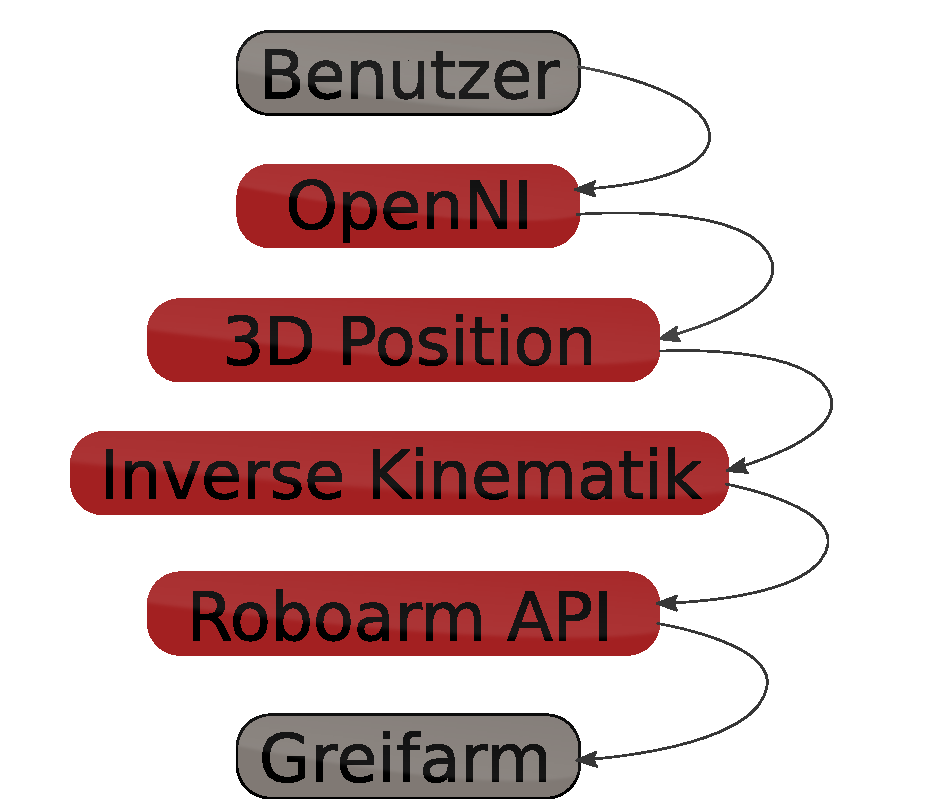
\includegraphics[width=\textwidth]{imgs/komponenten.pdf}
 }
 
%  \headerbox{}
%    {
%    name=z13,
%    column=2,
%    row=2,
%    below=headline,
%    textborder=none
%    }
%    {
%%\textbf{Komponenten}
%
% \lipsum[7-7]
% }

%%%%
%Inverse Kinematik
%%%
 \headerbox{\color{iwred}{\rule{1.0\textwidth}{4pt}}}{
 name=line2, 
% headerheight=0,
 column=0,
 row=2,
 span=3,
 below=z12,
 textborder=none
 }{}

    \headerbox{Inverse Kinematik}
    {
    name=z21,
    below=line2,
    column=0,
    row=2,
    textborder=none
    }
    {
        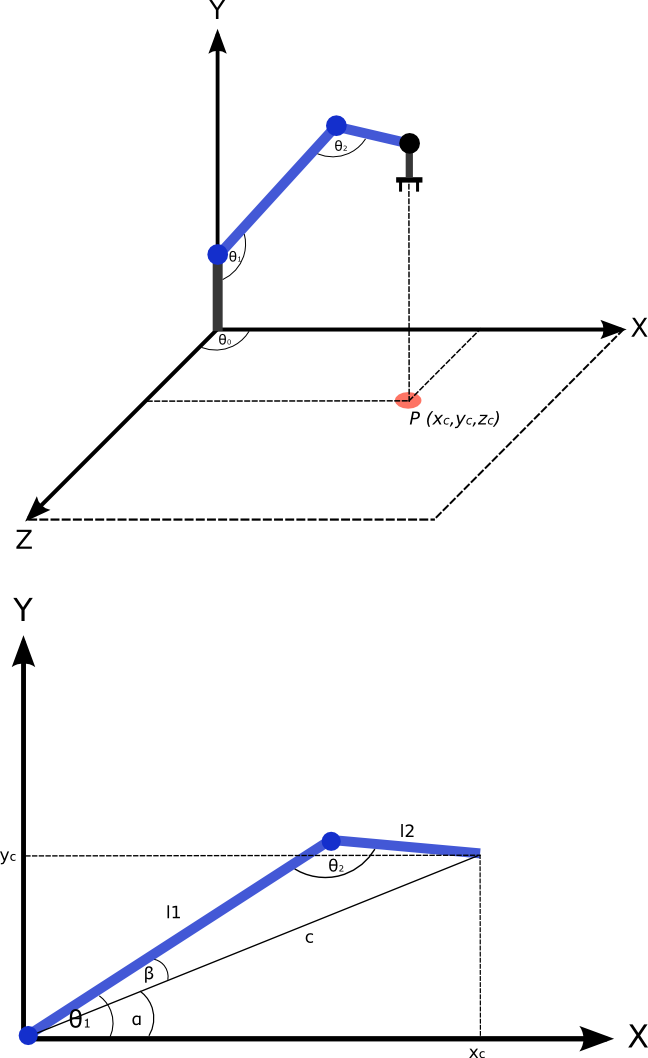
\includegraphics[width=\textwidth]{imgs/inverseKinematik.png}

 }
%%%%%%%%%%%%%%%%%%%%%%%%%%%%%%%%%%%%%%%%%%%%%%%%%%%%%%%%%%%%%%%%%%%%%%%%%%%%%%
\headerbox{}
    {
    name=z22,
    below=line2,
    column=1,
    row=2,
    textborder=none
    }
    {
	Die Inverse Kinematik hat die Aufgabe, aus der aktuellen 3D-Position des Spielers die Winkel des Roboterarms zu berechnen, damit der Greifer die Zielposition erreicht. Drei Winkel sind für dieses Problem zu berechnen: $\theta_0, \theta_1$ und $\theta_2$.
	\begin{enumerate}
	\item \textbf{$\theta_0$ - Drehung} 
\begin{eqnarray*}
	\theta_0 = atan2(z_c, x_c) \left[+ \pi \right]
	\end{eqnarray*}
	
	\item \textbf{$\theta_1$ - Beugung erstes Gelenk}
\begin{eqnarray*}
\theta_1 &=& \alpha + \beta \\
\theta_1 &=& atan2(y_c, z_c)\\ &+& atan2(E, \pm \sqrt{1-E^2}) \\
\cos \beta &=& \frac{l_1^2 + y_c^2 + z_c^2 - l_2^2}{2*l_1*\sqrt{z_c^2 + y_c^2}} := E 
	\end{eqnarray*}

	\item \textbf{$\theta_2$ - Beugung zweites Gelenk}
\begin{eqnarray*}
\theta_2 &=& atan2(D, \pm \sqrt{1-D^2}) \\
\cos \theta_2 &=& \frac{l_2^2 + l_1^2 - y_c^2 - z_c^2}{2*l_2*l_1} :=D
\end{eqnarray*}	
\end{enumerate}
	
Die Beugung und Drehung des Greifers übernimmt im Multi-Player Modus der zweite Spieler. Für eine einfache/intuitive Steuerung wird er im Single-Player automatisch senkrecht zur Arbeitsfläche ausgerichtet.
	  



 }
 \headerbox{Spiel-Modi}
    {
    name=z23,
    below=line2,
    column=2,
    row=2,
    textborder=none
    }
    {
 \textbf{Single-Player:}\vspace*{0.2cm} \\ 
Funktionen:
\begin{itemize}
\item Rechter Arm: Rotation um eigene Achse \& Beugung der Gelenke
\item Linker Arm: Öffnen/Schließen des Greifers
\item Greifer wird automatisch senkrecht zur Ebene ausgerichtet. \vspace*{0.2cm}\\
Winkelsumme im Viereck: \\ $\theta_3 = 360-((\theta_1-90)+\theta_2+90)$
\end{itemize}


 \textbf{Multi-Player:} \vspace*{0.2cm}\\
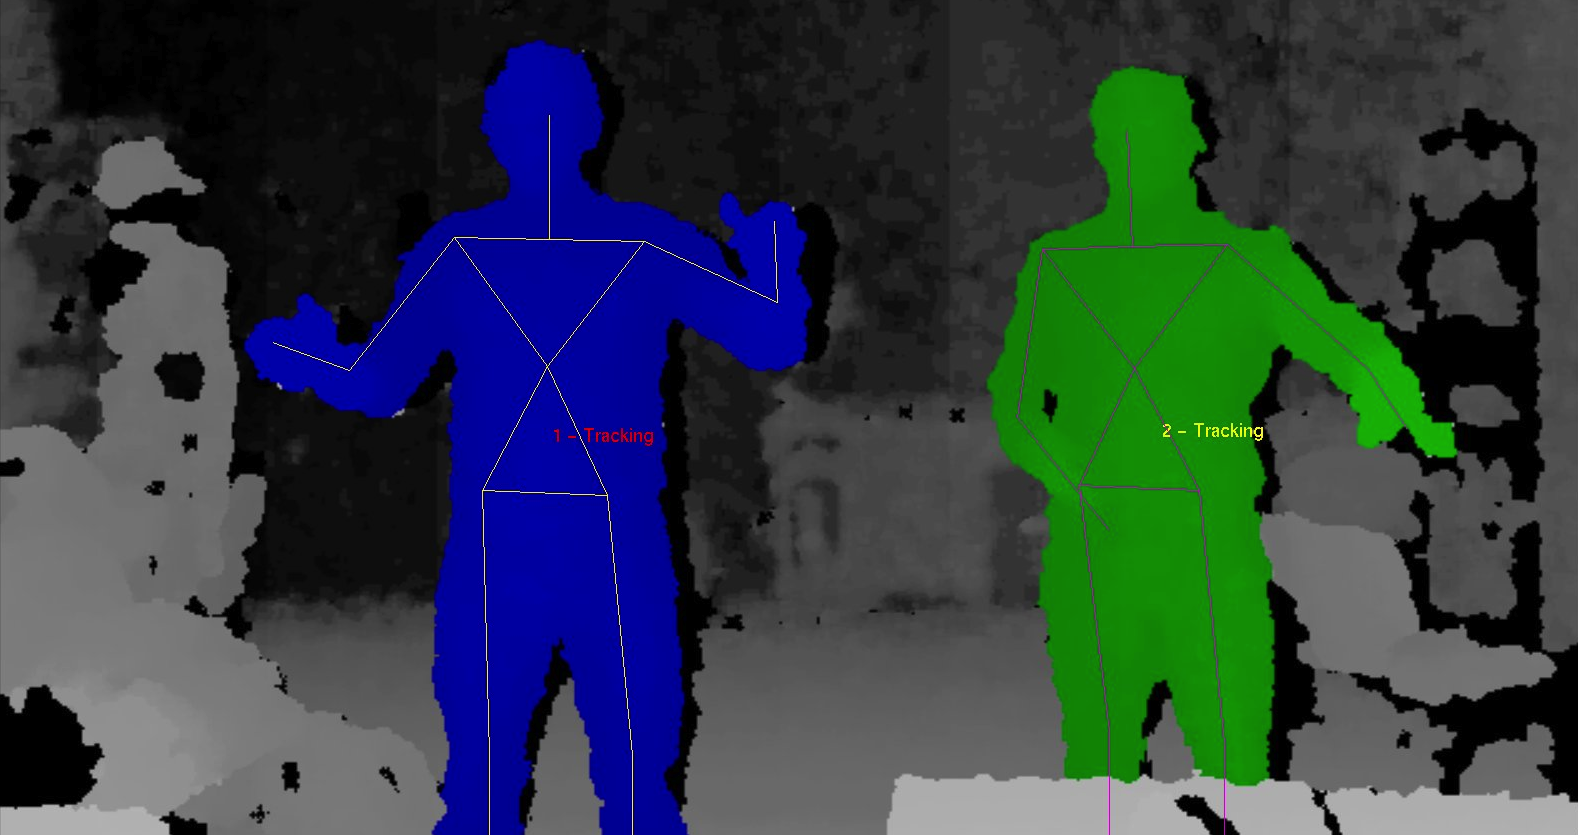
\includegraphics[width=\textwidth]{imgs/multiplayer_crop.png}\vspace*{0.05cm} \\
Funktionen: 
\begin{itemize}
\item 1. Spieler: Rotation \& Beugung des Greifarms ($\theta_0, \theta_1, \theta_2$).
\item 2. Spieler: Öffnen/Schließen \& Beugen des Greifers.
\end{itemize}
 }



 \headerbox{\color{iwred}{\rule{1.0\textwidth}{4pt}}}{
 name=line3, 
% headerheight=0,
below=z22,
 column=0,
 %row=3,
 span=3,
 textborder=none
 }
 {}

\headerbox{Team}
    {
    name=z31,
    below=line3,
    column=0,
    %row=2,
    textborder=none
    }
    {
    \textsf{\textbf{Manuel Dewald}\\
    Studiengang: Master Angewandte Informatik\\
	manuel.dewald@stud.uni-heidelberg.de
	}

 }
  \headerbox{}
    {
    name=z32,
    below=line3,
    column=1,
    %row=2,
    textborder=none
    }
    {
    \textsf{\textbf{Matthias Hummel}\\
    	Studiengang: Master Angewandte Informatik\\
	matthias.hummel@stud.uni-heidelberg.de 
	}
 }
 \headerbox{Betreuung}
    {
    name=z33,
    below=line3,
    column=2,
    %row=2,
    textborder=none
    }
    {
    \textsf{\textbf{Felix Aller} (felix.aller@iwr.uni-heidelberg.de),\\
    \textbf{Prof. Dr. Katja Mombaur}\\(kmombaur@uni-hd.de)}
  }


\end{poster}
\end{document}
